\section {Process}
This section describes the work and design challenges faced related to the PCB.
\subsection{Memory}
As discussed earlier, as one of our earliest design choices we chose 3 separate memories to allow overlap of
memory accesses. Since the requirements for the data/instruction memories differed in both size and word-width 
we wound up with not only separate, but also different chips for this purpose. The same choice meant we also
needed a separate memory for our \ac{VGA} controller, as that needed to read it's buffer as fast as possible
without interfering with the speed of the rest of the system. This called for a memory that was big enough to
hold atleast a full screen-frame, at 8-bit per pixel (since each pixel is an 8-bit greyscale pixel).

To reduce the possibility of having too slow data-access from the AVR, an extra memory was added to work as
a buffer for the AVR as well. This design choice was made {\em after} ordering, which meant that we had to choose from
the chips we had already ordered to fit this purpose. Since this was intended to carry data intended for the rest
of the system, and as the rest of the system is working with data in 8-bit bytes, we ended up using one of the
extra chips ordered as \ac{VGA} memory for this purpose.

\subsection {Schematics}

We decided to design the entire \ac{PCB} in one schematic, as the Festina Lente
report\TODO{Repeteres under} mentioned that using multiple schematics might give
some interesting issues.

A major downside of this approach was the fact that this completely serialized
our work on the Schematic, since we could not make concurrent changes to our
single document. This limited the parallelism of our workflow to one person at a
time working on the schematic.  In the meantime, the other people in the
\ac{PCB} group did whatever could be done without touching the
schematic. (Making footprints, verifying design, looking up parts and data
sheets) Since the schematic was the biggest amount of work, this produced
something of a bottleneck for the schematic work.

However, having the overall control of the entire thing in one document
did help to smooth out quite a few issues we met along the road. For instance,
we were having quite a few issues with netlabels. This was quite easy to
untangle when everything was in one document with 0 ports, as getting the
complete overview was very readable with this approach. We also avoided the need
to use any buses this way, although we did end up with one or two for the sake
of readability.

\TODO{Fill in a bit of details about pros for one-document vs multi.}  The
Festina Lente-report does mention that having multiple schematic documents
``made Altium issue a lot of warnings and errors during the design rule
check''\cite[p.~49]{berg2011festinalente}. Something we avoided from day one, as
we never attempted to use multiple schematics-documents. \TODO{Repeteres over}

The overall layout of the schematic is logically grouped ``geographically'', to
allow for easy reading of the schematic.

\subsubsection {Buses/Wirelabels}
We initially worked from the assumption that all pins should be connected to a
bus, and then that bus should be connected to the pins in the other end. This
gave us some issues with duplicate naming. After digging through quite a bit of
Altium documentation, we became assured that simply wire-labelling the pins
would create the necessary connections. This is because any pin/wire with the
same name as any other pin/wire will be connected by definition in Altium.

This arguably made for a less readable schematic, as the bus-connected solution
was quite a lot easier to follow when tracing. However, as our schematic still
is logically grouped, it is not very hard to find the correct connections even
without the busses drawn in. We are quite sure that given a logical overview of
which components are directly connected to each other, finding the various pins
that perform this connection should be trivial even without the busses/wires
drawn in.

\TODO{Overordnet forklaring av hvordan (JN: ???)}

\subsection {Routing}
\subsection {Routing}
\subsection {Routing}
\subsection {Routing}
\input{fig/pcb/routing}
We spent the entire final week before production working on the routing. In comparison, the energy group used only 2 days. There are quite a few possible reasons why we ended up using so much more time than them for this:

One of the reasons were simply that we were the first group to start routing. We thus got to fall into some gotcha-traps, with no one to warn us about them.

An example of such a trap was that we didn't set the correct Design Rules before auto-routing, until a few days into the week. This naturally didn't give us the routing that we wanted, and gave us a few headaches.

Related to this is the fact that we didn't experiment enough with different routing strategies. We wanted to reduce the number of vias, but went with the default routing in Altium. We then did quite an amount of manual routing to reduce the number of vias. Figure \ref{fig:removingvias-pcb} shows an example where we coupled together several pins to the same via going to the GND-layer. The amount of manual work could perhaps have been reduced by selecting the "Via Mixer" strategy instead.

\input{fig/pcb/pcb_removing_vias} \TODO{Write about this figure}

Another reason has to do with the difference between our designs. Where the other group had to route only 1 memory chip, we had 5. This naturally made the routing much more complex.

Initially we attempted auto routing. This took just around 12 minutes before constraints were set. And the better part of half an hour, after the constraints were set. This showed us quite a few issues that needed to be handled, and even more so when we finally got the constraints in.

\TODO{Fill in about the types of errors/warnings we got.}
\begin{itemize}
\item Constraints violations set wrong.
\item Power-plane net-labeled wrong.
\item Clearance constraints violated by Altium.
\item Short-circuiting vias.
\item Overlapping vias.
\item In general, the auto-routing started to produce violations.
\item more\ldots
\end{itemize}
\TODO{Silk-over-silk in USB/Lenna, errors we could ignore.}
\TODO{Scaling of board. (Should go elsewhere or not at all?)}

Initially we started with a board size chosen more or less at random, and picked something that seemed to fit the components comfortably with room to spare.

After laying out the components on the board, we noticed that the board had quite a bit of room left over. As this would be a waste of resources, we scaled the board down in size. We did this by moving the keep-out-borders inwards until the wasted space was removed, and then used the ``scale-to-fit-components''-tool in Altium, with the Keepout-border selected.

In the end we remapped some pins to increase physical proximity, and to untangle the amount of crossing wires. Although care was taken during this process, we accidentally happened to disconnect one pin in the schematic while reordering. We did notice this before production, and were able to correct the mistake by manually routing the connection. Finally, we did some manual routing to reduce the amount of unnecessary vias.


We spent the entire final week before production working on the routing. In comparison, the energy group used only 2 days. There are quite a few possible reasons why we ended up using so much more time than them for this:

One of the reasons were simply that we were the first group to start routing. We thus got to fall into some gotcha-traps, with no one to warn us about them.

An example of such a trap was that we didn't set the correct Design Rules before auto-routing, until a few days into the week. This naturally didn't give us the routing that we wanted, and gave us a few headaches.

Related to this is the fact that we didn't experiment enough with different routing strategies. We wanted to reduce the number of vias, but went with the default routing in Altium. We then did quite an amount of manual routing to reduce the number of vias. Figure \ref{fig:removingvias-pcb} shows an example where we coupled together several pins to the same via going to the GND-layer. The amount of manual work could perhaps have been reduced by selecting the "Via Mixer" strategy instead.

\begin{figure}[h]
  \centering
  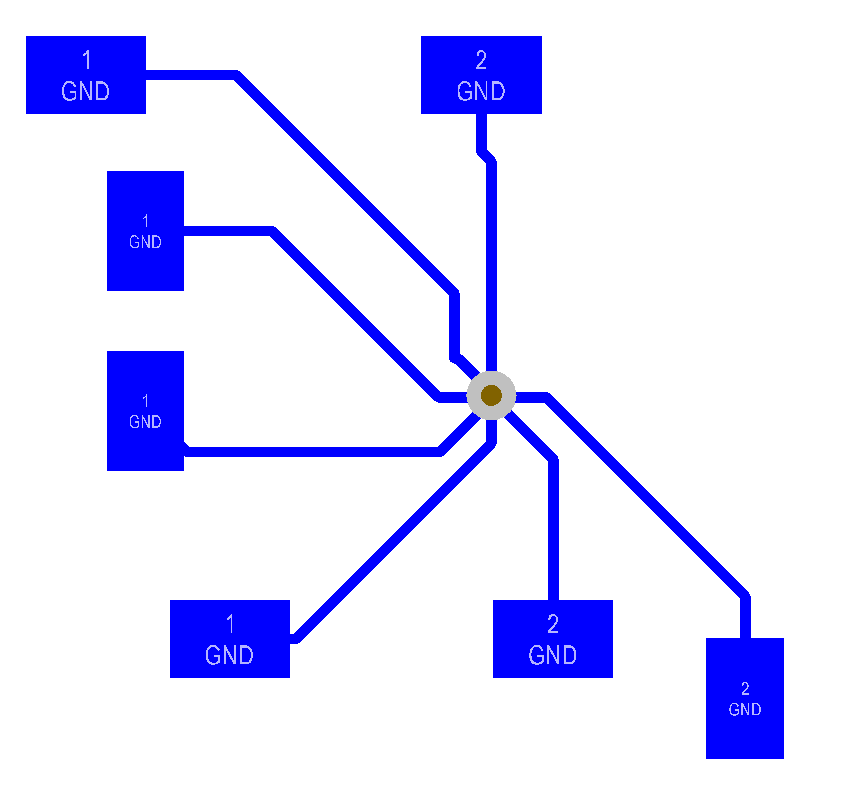
\includegraphics[width=0.8\textwidth]{fig/pcb/pcb_removing_vias.png}
  \caption{Removing vias}
  \label{fig:removingvias-pcb}
\end{figure}
 \TODO{Write about this figure}

Another reason has to do with the difference between our designs. Where the other group had to route only 1 memory chip, we had 5. This naturally made the routing much more complex.

Initially we attempted auto routing. This took just around 12 minutes before constraints were set. And the better part of half an hour, after the constraints were set. This showed us quite a few issues that needed to be handled, and even more so when we finally got the constraints in.

\TODO{Fill in about the types of errors/warnings we got.}
\begin{itemize}
\item Constraints violations set wrong.
\item Power-plane net-labeled wrong.
\item Clearance constraints violated by Altium.
\item Short-circuiting vias.
\item Overlapping vias.
\item In general, the auto-routing started to produce violations.
\item more\ldots
\end{itemize}
\TODO{Silk-over-silk in USB/Lenna, errors we could ignore.}
\TODO{Scaling of board. (Should go elsewhere or not at all?)}

Initially we started with a board size chosen more or less at random, and picked something that seemed to fit the components comfortably with room to spare.

After laying out the components on the board, we noticed that the board had quite a bit of room left over. As this would be a waste of resources, we scaled the board down in size. We did this by moving the keep-out-borders inwards until the wasted space was removed, and then used the ``scale-to-fit-components''-tool in Altium, with the Keepout-border selected.

In the end we remapped some pins to increase physical proximity, and to untangle the amount of crossing wires. Although care was taken during this process, we accidentally happened to disconnect one pin in the schematic while reordering. We did notice this before production, and were able to correct the mistake by manually routing the connection. Finally, we did some manual routing to reduce the amount of unnecessary vias.


We spent the entire final week before production working on the routing. In comparison, the energy group used only 2 days. There are quite a few possible reasons why we ended up using so much more time than them for this:

One of the reasons were simply that we were the first group to start routing. We thus got to fall into some gotcha-traps, with no one to warn us about them.

An example of such a trap was that we didn't set the correct Design Rules before auto-routing, until a few days into the week. This naturally didn't give us the routing that we wanted, and gave us a few headaches.

Related to this is the fact that we didn't experiment enough with different routing strategies. We wanted to reduce the number of vias, but went with the default routing in Altium. We then did quite an amount of manual routing to reduce the number of vias. Figure \ref{fig:removingvias-pcb} shows an example where we coupled together several pins to the same via going to the GND-layer. The amount of manual work could perhaps have been reduced by selecting the "Via Mixer" strategy instead.

\begin{figure}[h]
  \centering
  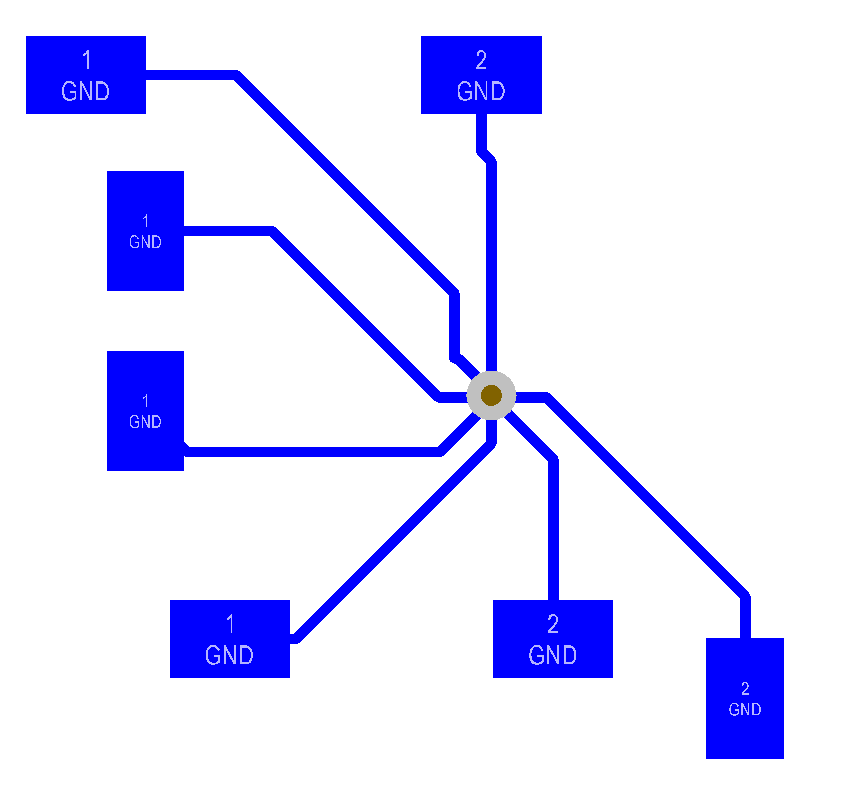
\includegraphics[width=0.8\textwidth]{fig/pcb/pcb_removing_vias.png}
  \caption{Removing vias}
  \label{fig:removingvias-pcb}
\end{figure}
 \TODO{Write about this figure}

Another reason has to do with the difference between our designs. Where the other group had to route only 1 memory chip, we had 5. This naturally made the routing much more complex.

Initially we attempted auto routing. This took just around 12 minutes before constraints were set. And the better part of half an hour, after the constraints were set. This showed us quite a few issues that needed to be handled, and even more so when we finally got the constraints in.

\TODO{Fill in about the types of errors/warnings we got.}
\begin{itemize}
\item Constraints violations set wrong.
\item Power-plane net-labeled wrong.
\item Clearance constraints violated by Altium.
\item Short-circuiting vias.
\item Overlapping vias.
\item In general, the auto-routing started to produce violations.
\item more\ldots
\end{itemize}
\TODO{Silk-over-silk in USB/Lenna, errors we could ignore.}
\TODO{Scaling of board. (Should go elsewhere or not at all?)}

Initially we started with a board size chosen more or less at random, and picked something that seemed to fit the components comfortably with room to spare.

After laying out the components on the board, we noticed that the board had quite a bit of room left over. As this would be a waste of resources, we scaled the board down in size. We did this by moving the keep-out-borders inwards until the wasted space was removed, and then used the ``scale-to-fit-components''-tool in Altium, with the Keepout-border selected.

In the end we remapped some pins to increase physical proximity, and to untangle the amount of crossing wires. Although care was taken during this process, we accidentally happened to disconnect one pin in the schematic while reordering. We did notice this before production, and were able to correct the mistake by manually routing the connection. Finally, we did some manual routing to reduce the amount of unnecessary vias.


We spent the entire final week before production working on the routing. In comparison, the energy group used only 2 days. There are quite a few possible reasons why we ended up using so much more time than them for this:

One of the reasons were simply that we were the first group to start routing. We thus got to fall into some gotcha-traps, with no one to warn us about them.

An example of such a trap was that we didn't set the correct Design Rules before auto-routing, until a few days into the week. This naturally didn't give us the routing that we wanted, and gave us a few headaches.

Related to this is the fact that we didn't experiment enough with different routing strategies. We wanted to reduce the number of vias, but went with the default routing in Altium. We then did quite an amount of manual routing to reduce the number of vias. The amount of manual work could perhaps have been reduced by selecting the "Via Mixer" strategy instead.

\TODO{Insert "via-hub" figure here}

Another reason has to do with the difference between our designs. Where the other group had to route only 1 memory chip, we had 5. This naturally made the routing much more complex.

Initially we attempted autorouting. This took just around 12 minutes before constraints were set. And the better part of half an hour, after the constraints were set. This showed us quite a few issues that needed to be handled, and even more so when we finally got the constraints in.

\TODO{Fill in about the types of errors/warnings we got.}
\begin{itemize}
\item Constraints violations set wrong.
\item Power-plane net-labeled wrong.
\item Clearance constraints violated by Altium.
\item Short-circuiting vias.
\item Overlapping vias.
\item In general, the auto-routing started to produce violations.
\item more\ldots
\end{itemize}
\TODO{Silk-over-silk in USB/Lenna, errors we could ignore.}
\TODO{Scaling of board. (Should go elsewhere or not at all?)}

Initially we started with a board size chosen more or less at random, and picked something that seemed to fit the components comfortably with room to spare.

After laying out the components on the board, we noticed that the board had quite a bit of room left over. As this would be a waste of resources, we scaled the board down in size. We did this by moving the keep-out-borders inwards until the wasted space was removed, and then used the ``scale-to-fit-components''-tool in Altium, with the Keepout-border selected.

In the end we remapped some pins to increase physical proximity, and to untangle the amount of crossing wires. Although care was taken during this process, we accidentally happened to disconnect one pin in the schematic while reordering. We did notice this before production, and were able to correct the mistake by manually routing the connection. Finally, we did some manual routing to reduce the amount of unneccessary vias.

\subsection{Soldering}
After that we started soldering the AVR. Getting the AVR in place was particularly difficult,
but after asking Tufte, we lent a glue stick to put some glue on. The increased friction helped keeping the AVR in place during soldering.

After about a days work we managed to completely destroy a pin on the AVR,
therefore we had to start from scratch on a new board. On this new board we
started with the AVR and \ac{FPGA}, as they were the hardest components to
solder. After each side on the AVR and \ac{FPGA}, we tested for short
circuits. As none were found, we moved on to the power supply, as well as
\acp{JTAG}, FLASH and \acp{LED}. In order to check the \ac{PCB} was working, the
AVR and \ac{FPGA} groups tested the \ac{PCB} board without the capacitors, after
both groups tested that they could connect to the AVR and \ac{FPGA}
respectively, we began to solder the rest part of the \ac{PCB}.

